
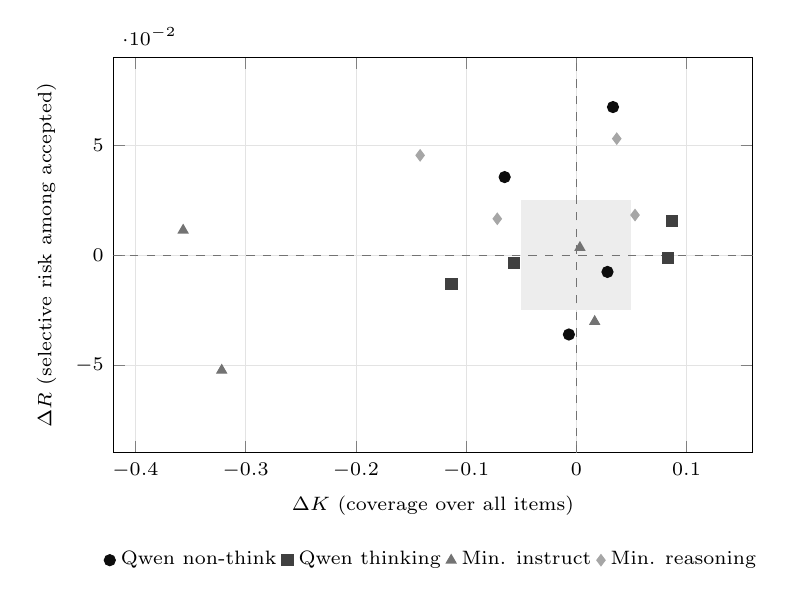
\begin{tikzpicture}
\begin{axis}[
  width=0.80\textwidth, height=6.6cm,
  xlabel={$\Delta K$ (coverage over all items)},
  ylabel={$\Delta R$ (selective risk among accepted)},
  xmin=-0.42, xmax=0.16, ymin=-0.09, ymax=0.09,
  tick label style={font=\scriptsize}, label style={font=\scriptsize},
  legend style={font=\scriptsize, at={(0.5,-0.22)}, anchor=north, legend columns=4, draw=none},
  grid=major, grid style={gray!22,very thin}]
\fill[black!7] (axis cs:-0.05,-0.025) rectangle (axis cs:0.05,0.025);
\draw[black!55,dashed] (axis cs:-0.42,0) -- (axis cs:0.16,0);
\draw[black!55,dashed] (axis cs:0,-0.09) -- (axis cs:0,0.09);
\addplot[only marks, mark=*, mark size=2.0pt, color=black!95] coordinates {(0.0333,0.0675) (-0.0067,-0.0361) (-0.0650,0.0356) (0.0283,-0.0076)};
\addlegendentry{Qwen non-think}
\addplot[only marks, mark=square*, mark size=2.0pt, color=black!75] coordinates {(0.0867,0.0157) (-0.1133,-0.0132) (-0.0567,-0.0037) (0.0833,-0.0011)};
\addlegendentry{Qwen thinking}
\addplot[only marks, mark=triangle*, mark size=2.0pt, color=black!55] coordinates {(-0.3217,-0.0524) (0.0167,-0.0302) (-0.3567,0.0114) (0.0033,0.0035)};
\addlegendentry{Min. instruct}
\addplot[only marks, mark=diamond*, mark size=2.0pt, color=black!35] coordinates {(-0.0717,0.0166) (0.0533,0.0183) (0.0367,0.0531) (-0.1417,0.0455)};
\addlegendentry{Min. reasoning}
\end{axis}
\end{tikzpicture}
